\documentclass[a4paper, 12pt]{article}
\usepackage{authblk}
\renewcommand{\Affilfont}{\footnotesize}
\title{Cabinet under Pressure: Survival Analysis of Peru’s Prime Ministers Since 1980}
\author[1,2]{ Jose Manuel Magallanes }
\affil[1]{PULSO -Institute of Social Analytics and Strategic Intelligence and Department of Social Sciences, Pontificia Universidad Catolica del Peru, San Miguel 15088, Lima, Peru}
\affil[2]{University of Massachusetts-Amherst; University of Washington -Seattle; and Universidad Nacional Mayor de San Marcos-Lima}
\affil[*]{Corresponding author: jmagallanes@pucp.edu.pe}


\date{\today}  %% manually: \date{March 6, 2025} 
\usepackage[natbibapa]{apacite} %% for bibliography
\usepackage{rotating, graphicx} %% for rotating tables
\usepackage{adjustbox} % size of plots and tables
\usepackage{chngcntr}% section numbering
\usepackage{amssymb}
\counterwithin{table}{section}\counterwithin{figure}{section}
\usepackage{Sweave}
\begin{document} % every "begin: needs and "end"
\Sconcordance{concordance:WorkInR_forPrinter.tex:WorkInR_forPrinter.Rnw:1 17 1 1 0 34 %
1 1 2 1 0 2 1 1 3 2 0 1 6 22 0 1 2 10 1 1 13 11 1 1 18 16 0 1 3 12 1 1 %
12 1 2 14 1 1 15 23 0 1 2 7 1 1 11 1 2 12 1 1 8 24 0 1 2 9 1 1 9 4 1 1 %
7 29 0 1 2 18 1 1 16 3 1 1 3 1 2 10 1 1 7 1 2 21 1}

\maketitle 
\begin{abstract}
This study examines the political durability of Peru’s Prime Ministers (Presidente del Consejo de Ministros, PCM) since the country’s democratic return in 1980. Using survival analysis, we explore how political context, institutional conditions, and crisis dynamics shape the tenure of these key presidential appointees. Through a Cox proportional hazards model, we test the influence of presidential popularity, legislative fragmentation, cabinet reshuffles, and regime instability on the risk of early dismissal or resignation. The results illuminate how informal power-sharing and institutional fragility influence executive coordination in a hyper-presidential regime.
\end{abstract}


\section*{Introduction} % * to unnumber

The median tenure of a Peruvian Prime Minister (PCM) since 1980 is 254 days (around 8 months), yet variation is striking. \'{A}ntero Flores\-Ar\'{a}oz lasted only six days in November 2020, whereas Manuel Ulloa served 864 days in the early 1980s and Jorge del Castillo survived 805 days during Alan Garc\'{i}a\'s second term. Dispersion persists even within a single presidential period: three PCMs held the post during Pedro Castillo\'s first five months, while Alberto Ot\'{a}rola remained in office for 440 days under Dina Boluarte. This inconsistency under ostensibly similar institutional rules raises a central puzzle: Which political, institutional, and situational factors condition the durability of Peru\'s Prime Ministers?

Although the Constitution describes the PCM merely as the president’s first minister—responsible for countersigning decrees and coordinating the cabinet—practice since 1980 indicates that the office routinely performs head-of-government functions: drafting the policy agenda, negotiating confidence votes, and representing the executive in congressional interpellations. The PCM thus acts as the president’s chief political shield. During normal times, the office facilitates legislative compromise and signals technocratic competence; in crises, it functions as a “circuit-breaker,” a high-visibility scapegoat whose dismissal absorbs congressional anger and preserves presidential tenure. Analysing the determinants of PCM survival therefore illuminates how Peru’s hyper-presidential system manages accountability, blame assignment, and policy coordination in the absence of strong parties.



\section{Background}\label{explo-tables} % label for crossref

Legal foundations (Art.124, 1993 Constitution): The PCM is named by the President but becomes fully operative only after the Council of Ministers receives a congressional vote of confidence (Art.130). Article 124 establishes five formal powers that lift the office above an ordinary minister: (1) countersigning every presidential decree and law, thereby granting legal validity; (2) convening and presiding over the Council of Ministers when the President is absent; (3) coordinating sectoral policies and monitoring implementation across ministries; (4) presenting the government’s general policy and annual budget bill to Congress; and (5) proposing—on behalf of the Council—votes of confidence or requesting the President to dissolve Congress after two denials. Taken together, these clauses make the PCM the linchpin between executive decree authority and legislative oversight, subject to individual censure (Art.132) and collective cabinet responsibility. This constitutional design explains why dismissing the PCM can defuse political crises without toppling the President.
Informal evolution: From symbolic coordinator to key political operator. In the early 1980s the PCM was largely a symbolic co‑signatory—Manuel Ulloa chaired cabinet meetings but real bargaining occurred directly between President Belaúnde and party caucuses. Two changes transformed the post:
Fujimori’s executive re‑engineering (1990‑2000): frequent decree lawmaking and the 1992 Constitution concentrated agenda control in the Palace. The PCM became the de facto gatekeeper of emergency decrees, crisis communication, and IMF negotiations. Guillermo Larco Cox’s 1989 and Hurtado Miller’s 1990 tenures were early signs; by 1995 Dante Córdova was publicly branded “Premier”, marking a rhetorical shift from coordinator to operator.

Confidence‑vote politics after 2000: Article 130 requires each new Council to obtain a congressional vote of confidence, but presidents have repeatedly weaponised the PCM to reset relations with an antagonistic Congress—e.g., Salomón Lerner (2011), César Villanueva (2013, 2018), Pedro Cateriano(2020). The PCM now drafts policy speeches, counts votes, and negotiates floor time, acting as a quasi‑prime minister in a party‑fragmented legislature.

Consequently, career technocrats and seasoned politicians alike view the PCM as the highest non‑presidential prize—yet also the first political “fuse” to blow when scandals erupt. Our duration data confirm this duality: the office’s power has grown, but so has its volatility, illustrating the gap between formal rules and informal political practice.

Role during key periods:

\begin{enumerate}
    \item Democratic transition (1980–1989): Under Belaúnde and García I, the PCM was chiefly a coalition‑balancing broker: Manuel Ulloa, Fernando Schwalb, and Luis Alva Castro used the office to mediate between the president and newly elected party caucuses, but limited decree use kept the post largely symbolic. Average tenure was around 450 days.
    \item Fujimori era (1990–2000): Executive decree authority and the 1992 Constitution turned the PCM into the president’s operational shield. PMs like Hurtado Miller (199 days) and Pandolfi (792 days across two spells) managed IMF talks and emergency legislation, yet were dismissed when inflation, corruption, or congressional frictions peaked, thus underscoring the role as sacrificial buffer.
    \item Post‑2000 democratic turbulence: With weak parties and fragmented congresses, the PCM became the pivot for confidence‑vote politics. Thirty‑four different PMs have served since 2001, median tenure just 232 days. Presidents Toledo, Humala, Vizcarra, Castillo, and Boluarte each used rapid PCM turnover to re‑negotiate legislative support—e.g., Cateriano’s 22‑day tenure (2020) followed by Martos’s 96 days as the executive searched for votes of confidence.
\end{enumerate}


\begin{Schunk}
\begin{Sinput}
> library(knitr)
> library(magrittr)
> library(kableExtra)
> # Toy example 
> df <- data.frame(x = c(1:3), 
+              y = c(4:6))
> # Using kableExtra 
> df %>%
+     kbl(caption = "Example", # Adding caption  
+         format = "latex") %>% # Output format = latex 
+     kable_classic(html_font = "Cambria") # Font = Cambria 
\end{Sinput}
\begin{table}
\centering
\caption{Example}
\centering
\begin{tabular}[t]{r|r}
\hline
x & y\\
\hline
1 & 4\\
\hline
2 & 5\\
\hline
3 & 6\\
\hline
\end{tabular}
\end{table}\end{Schunk}


I will soon use cross-ref.I will soon use cross-ref.I will soon use cross-ref.I will soon use cross-ref. I will soon use cross-ref. I will soon use cross-ref.I will soon use cross-ref.I will soon use cross-ref.I will soon use cross-ref.I will soon use cross-ref. I will soon use cross-ref. I will soon use cross-ref.
%cross-ref coming

%cross-ref coming
I will soon use cross-ref.I will soon use cross-ref: as we see in Section \ref{catexplor}.

% a chunk hidden (echo=FALSE) with some setup
% chunk has its own name 


\subsection{Exploring Categorical Data}\label{catexplor}

Here, I continue doing this nice work, I hope you like it and read it. It has been a very hard work.Here, I continue doing this nice work, I hope you like it and read it. It has been a very hard work.Here, I continue doing this nice work, I hope you like it and read it. It has been a very hard work.Here, I continue doing this nice work, I hope you like it and read it. It has been a very hard work.Here, I continue doing this nice work, I hope you like it and read it. It has been a very hard work.Here, I continue doing this nice work, I hope you like it and read it. It has been a very hard work.

I hope you like it and read it. It has been a very hard work.Here, I continue doing this nice work, I hope you like it and read it. It has been a very hard work.Here, I continue doing this nice work, I hope you like it and read it. It has been a very hard work.Here, I continue doing this nice work, I hope you like it and read it. It has been a very hard work.Here, I continue doing this nice work, I hope you like it and read it. It has been a very hard work.

You can see the statistics of a categorical variable in Table \ref{catexploreTable}.

%the chunk name is NOT used in cross-ref for table.
%Table is created and displayed.

\begin{table}[!h]
\centering
\caption{This is a table\label{catexploreTable}}
\centering
\begin{tabular}[t]{l|r|r|r}
\hline
Democracy Level & count & pct & pct\_cumm\\
\hline
Authoritarian & 57 & 36.08 & 36.08\\
\hline
Hybrid regime & 32 & 20.25 & 56.33\\
\hline
Flawed democracy & 50 & 31.65 & 87.97\\
\hline
Full democracy & 19 & 12.03 & 100.00\\
\hline
\end{tabular}
\end{table}

%%%%%%

You can see this variable plotted in Figure \ref{catBarplot} on page \pageref{catBarplot}.

% NO need for figure caption in chunk header.
% Object will be created BUT NOT plotted
% the chunk name IS NOT used in cross-ref for figure

\begin{figure}[h]
\centering
\begin{adjustbox}{width=7cm,height=5cm} %resize
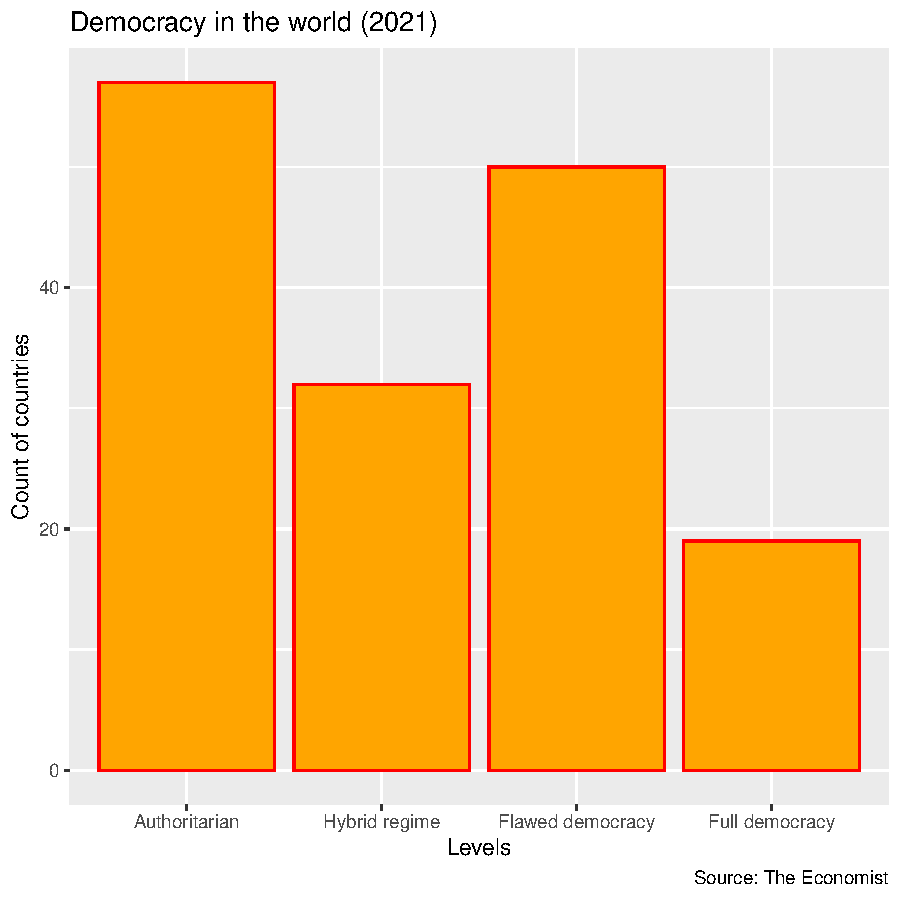
\includegraphics{WorkInR_forPrinter-catBarplot}
\end{adjustbox}
\caption{Press Freedom Index in the World}  %title
\label{catBarplot} % for cross-ref
\end{figure}



\subsection{Exploring Numerical Data}\label{numexplo}

Here, I continue doing this nice work, I hope you like it and read it. It has been a very hard work.Here, I continue doing this nice work, I hope you like it and read it. It has been a very hard work.Here, I continue doing this nice work, I hope you like it and read it. It has been a very hard work.Here, I continue doing this nice work, I hope you like it and read it. It has been a very hard work.Here, I continue doing this nice work, I hope you like it and read it. It has been a very hard work.Here, I continue doing this nice work, I hope you like it and read it. It has been a very hard work.Here, I continue doing this nice work, I hope you like it and read it. It has been a very hard work.Here, I continue doing this nice work, I hope you like it and read it. It has been a very hard work.Here, I continue doing this nice work, I hope you like it and read it. It has been a very hard work.

Here, I continue doing this nice work, I hope you like it and read it. It has been a very hard work.Here, I continue doing this nice work, I hope you like it and read it. It has been a very hard work.Here, I continue doing this nice work, I hope you like it and read it. It has been a very hard work.Here, I continue doing this nice work, I hope you like it and read it. It has been a very hard work.Here, I continue doing this nice work, I hope you like it and read it. It has been a very hard work.Here, I continue doing this nice work, I hope you like it and read it. It has been a very hard work.Here, I continue doing this nice work, I hope you like it and read it. It has been a very hard work.Here, I continue doing this nice work, I hope you like it and read it. It has been a very hard work.Here, I continue doing this nice work, I hope you like it and read it. It has been a very hard work.

Here, I continue doing this nice work, I hope you like it and read it. It has been a very hard work.Here, I continue doing this nice work, I hope you like it and read it. It has been a very hard work.

% Table created by stargazer v.5.2.3 by Marek Hlavac, Social Policy Institute. E-mail: marek.hlavac at gmail.com
% Date and time: Fri, May 09, 2025 - 14:54:53
\begin{table}[!htbp] \centering 
  \caption{Stat summary for numeric vars} 
  \label{summaryNumeric} 
\scriptsize 
\begin{tabular}{@{\extracolsep{5pt}}lccccccc} 
\\[-1.8ex]\hline 
\hline \\[-1.8ex] 
Statistic & \multicolumn{1}{c}{N} & \multicolumn{1}{c}{Mean} & \multicolumn{1}{c}{St. Dev.} & \multicolumn{1}{c}{Min} & \multicolumn{1}{c}{Pctl(25)} & \multicolumn{1}{c}{Pctl(75)} & \multicolumn{1}{c}{Max} \\ 
\hline \\[-1.8ex] 
HumanDevelopmentIndex & 158 & 0.72 & 0.16 & 0.39 & 0.59 & 0.85 & 0.96 \\ 
LifeExpectancyAtBirth & 158 & 71.17 & 7.89 & 52.53 & 65.05 & 76.82 & 85.47 \\ 
ExpectedYearsOfSchooling & 158 & 13.60 & 2.98 & 6.96 & 11.51 & 15.70 & 21.05 \\ 
MeanYearsOfSchooling & 158 & 8.96 & 3.32 & 2.11 & 6.05 & 11.64 & 14.09 \\ 
GrossNationalIncomePerCapita & 158 & 20,126.60 & 20,390.02 & 731.79 & 4,552.38 & 30,106.04 & 90,918.64 \\ 
Overallscore & 158 & 5.26 & 2.29 & 0.32 & 3.21 & 7.00 & 9.75 \\ 
Electoralprocessandpluralism & 158 & 5.60 & 3.81 & 0.00 & 1.44 & 9.17 & 10.00 \\ 
Functioningofgovernment & 158 & 4.58 & 2.58 & 0.00 & 2.50 & 6.43 & 9.64 \\ 
Politicalparticipation & 158 & 5.40 & 1.95 & 0.00 & 3.89 & 6.67 & 10.00 \\ 
Politicalculture & 158 & 5.35 & 1.82 & 1.25 & 3.75 & 6.25 & 10.00 \\ 
Civilliberties & 158 & 5.37 & 2.66 & 0.00 & 3.24 & 7.65 & 9.71 \\ 
\hline \\[-1.8ex] 
\end{tabular} 
\end{table} 
% Use of R object inline
In the Table \ref{summaryNumeric}, you realize that the mean of HDI is {\bf0.72}. It would be good to see a boxplot, check Figure \ref{numBoxplot} below.


\begin{figure}[h]
\centering
\begin{adjustbox}{width=12cm,height=8.5cm,clip,trim=0cm 0.5cm 0cm 0cm} 
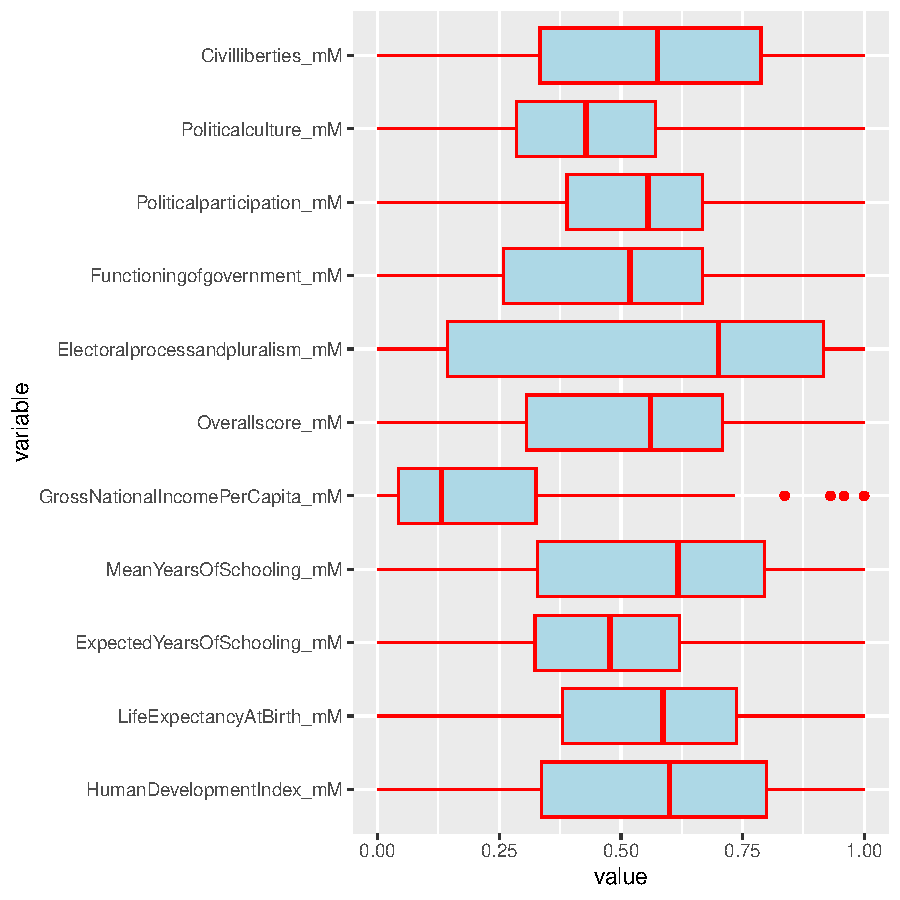
\includegraphics{WorkInR_forPrinter-numBoxplot}
\end{adjustbox}
\caption{The nice boxplots}  
\label{numBoxplot} 
\end{figure}

%%%%% A citation: author(year)

Boxplots were introduced by \citet{tukey_exploratory_1977}.

You can also flip the Table \ref{summaryNumeric}, as shown in Table \ref{summaryNumeric-flip}.



% Table created by stargazer v.5.2.3 by Marek Hlavac, Social Policy Institute. E-mail: marek.hlavac at gmail.com
% Date and time: Fri, May 09, 2025 - 14:54:54
% Requires LaTeX packages: rotating 
\begin{sidewaystable}[!htbp] \centering 
  \caption{Stat summary for numeric vars (flipped)} 
  \label{summaryNumeric-flip} 
\scriptsize 
\begin{tabular}{@{\extracolsep{5pt}}lccccccc} 
\\[-1.8ex]\hline 
\hline \\[-1.8ex] 
Statistic & \multicolumn{1}{c}{N} & \multicolumn{1}{c}{Mean} & \multicolumn{1}{c}{St. Dev.} & \multicolumn{1}{c}{Min} & \multicolumn{1}{c}{Pctl(25)} & \multicolumn{1}{c}{Pctl(75)} & \multicolumn{1}{c}{Max} \\ 
\hline \\[-1.8ex] 
HumanDevelopmentIndex & 158 & 0.72 & 0.16 & 0.39 & 0.59 & 0.85 & 0.96 \\ 
LifeExpectancyAtBirth & 158 & 71.17 & 7.89 & 52.53 & 65.05 & 76.82 & 85.47 \\ 
ExpectedYearsOfSchooling & 158 & 13.60 & 2.98 & 6.96 & 11.51 & 15.70 & 21.05 \\ 
MeanYearsOfSchooling & 158 & 8.96 & 3.32 & 2.11 & 6.05 & 11.64 & 14.09 \\ 
GrossNationalIncomePerCapita & 158 & 20,126.60 & 20,390.02 & 731.79 & 4,552.38 & 30,106.04 & 90,918.64 \\ 
Overallscore & 158 & 5.26 & 2.29 & 0.32 & 3.21 & 7.00 & 9.75 \\ 
Electoralprocessandpluralism & 158 & 5.60 & 3.81 & 0.00 & 1.44 & 9.17 & 10.00 \\ 
Functioningofgovernment & 158 & 4.58 & 2.58 & 0.00 & 2.50 & 6.43 & 9.64 \\ 
Politicalparticipation & 158 & 5.40 & 1.95 & 0.00 & 3.89 & 6.67 & 10.00 \\ 
Politicalculture & 158 & 5.35 & 1.82 & 1.25 & 3.75 & 6.25 & 10.00 \\ 
Civilliberties & 158 & 5.37 & 2.66 & 0.00 & 3.24 & 7.65 & 9.71 \\ 
\hline \\[-1.8ex] 
\end{tabular} 
\end{sidewaystable} 
\pagebreak



%%%%
\section{My Regression}\label{regre}

Several times we need regression. This is a nice summary for two regressions, as shown in Table \ref{regsPrint}:






% Table created by stargazer v.5.2.3 by Marek Hlavac, Social Policy Institute. E-mail: marek.hlavac at gmail.com
% Date and time: Fri, May 09, 2025 - 14:54:54
\begin{table}[!htbp] \centering 
  \caption{Models for HDI} 
  \label{regsPrint} 
\begin{tabular}{@{\extracolsep{5pt}}lcc} 
\\[-1.8ex]\hline 
\hline \\[-1.8ex] 
 & \multicolumn{2}{c}{\textit{Dependent variable:}} \\ 
\cline{2-3} 
\\[-1.8ex] & \multicolumn{2}{c}{Human Development} \\ 
\\[-1.8ex] & (1) & (2)\\ 
\hline \\[-1.8ex] 
 Bureaucracy & 0.042$^{***}$ & 0.036$^{***}$ \\ 
  & (0.003) & (0.005) \\ 
  & & \\ 
 Participation &  & 0.013$^{**}$ \\ 
  &  & (0.006) \\ 
  & & \\ 
 Constant & 0.526$^{***}$ & 0.488$^{***}$ \\ 
  & (0.018) & (0.026) \\ 
  & & \\ 
\hline \\[-1.8ex] 
Observations & 158 & 158 \\ 
Log Likelihood & 121.396 & 123.419 \\ 
Akaike Inf. Crit. & $-$238.792 & $-$240.837 \\ 
\hline 
\hline \\[-1.8ex] 
\textit{Note:}  & \multicolumn{2}{r}{$^{*}$p$<$0.1; $^{**}$p$<$0.05; $^{***}$p$<$0.01} \\ 
\end{tabular} 
\end{table} 
I hope you like what you see in the Table \ref{regsPrint}. 

You can learn more on regression in other book \citep[150-160]{petrie_introduction_2016}

%%%%


\section{Other plots}\label{otherPlots}


\subsection{A map}\label{mapPlot}

Let me show a nice map.Let me show a nice map.Let me show a nice map.Let me show a nice map.Let me show a nice map.Let me show a nice map.Let me show a nice map.Let me show a nice map.Let me show a nice map.Let me show a nice map.Let me show a nice map.Let me show a nice map.

Let me show a nice map.Let me show a nice map.Let me show a nice map.Let me show a nice map.Let me show a nice map.Let me show a nice map.Let me show a nice map.Let me show a nice map.Let me show a nice map.Let me show a nice map.Let me show a nice map.Let me show a nice map.

Let me show a nice map.Let me show a nice map.Let me show a nice map.Let me show a nice map.Let me show a nice map.Let me show a nice map.Let me show a nice map.Let me show a nice map.Let me show a nice map.Let me show a nice map.Let me show a nice map.Let me show a nice map in Figure \ref{plot-cityMap}.


\begin{figure}[h]
\centering
\begin{adjustbox}{width=10cm,height=10cm} 
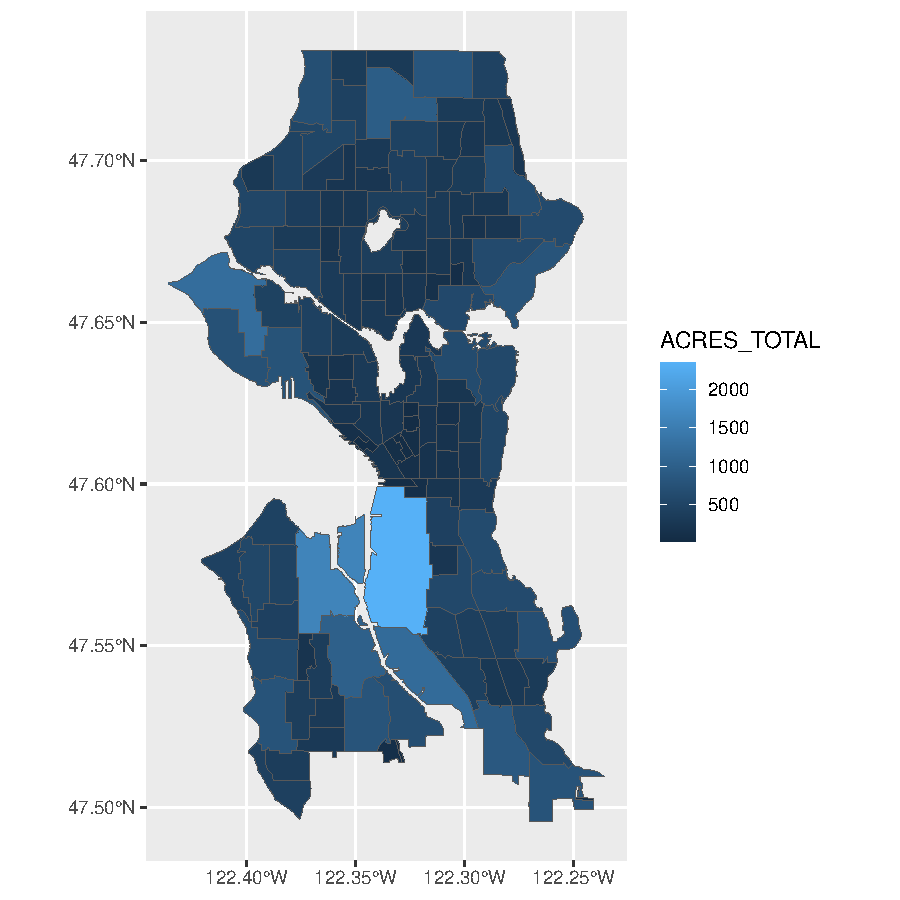
\includegraphics{WorkInR_forPrinter-plot-cityMap}
\end{adjustbox}
\caption{Plot numeric colums.}  
\label{plot-cityMap} 
\end{figure}

Figure \ref{plot-cityMap} uses only one layer. Let's add another layer in the next map. Here, I continue doing this nice work, I hope you like it and read it. It has been a very hard work.Here, I continue doing this nice work, I hope you like it and read it. It has been a very hard work.Here, I continue doing this nice work, I hope you like it and read it. It has been a very hard work.Here, I continue doing this nice work, I hope you like it and read it.  Here, I continue doing this nice work, I hope you like it and read it. It has been a very hard work.Here, I continue doing this nice work, I hope you like it and read it. It has been a very hard work.Here, I continue doing this nice work, I hope you like it and read it. It has been a very hard work.Here, I continue doing this nice work, I hope you like it and read it.


\begin{figure}[h]
\centering
\begin{adjustbox}{width=10cm,height=10cm} 
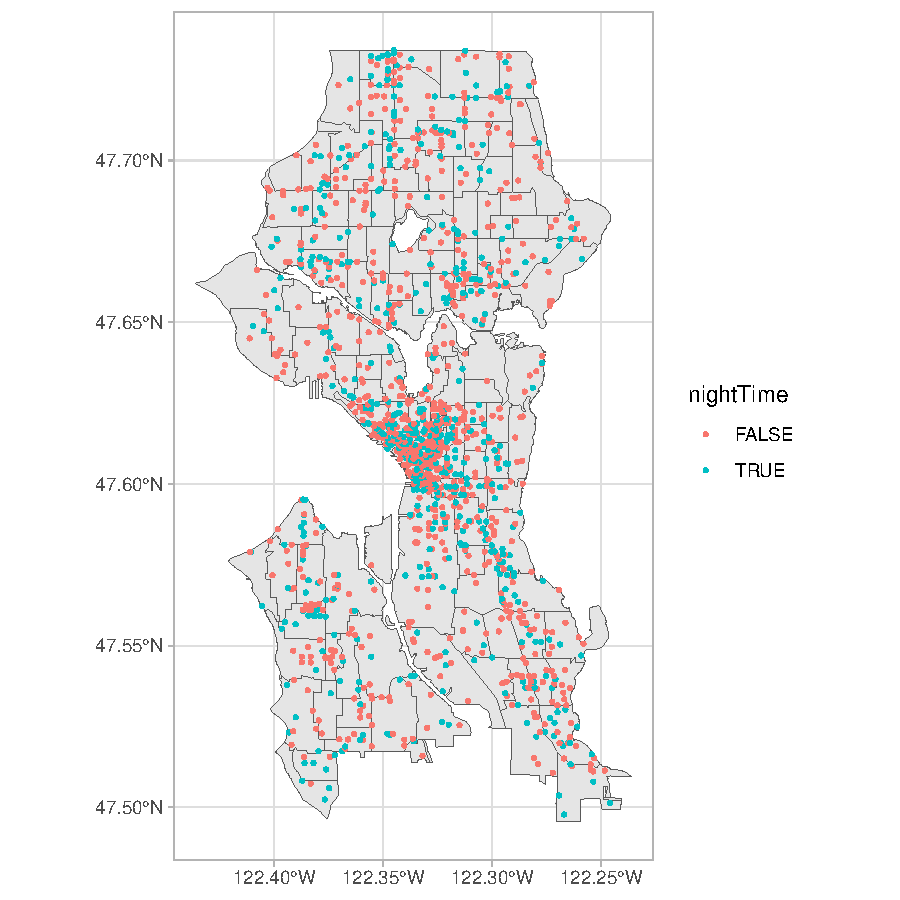
\includegraphics{WorkInR_forPrinter-plot-911Map}
\end{adjustbox}
\caption{Calls to 911 by time of day.}  
\label{plot-911Map} 
\end{figure}

You can see that Figure \ref{plot-911Map} actually uses one map on top of the other. 
Here, I continue doing this nice work, I hope you like it and read it. It has been a very hard work.Here, I continue doing this nice work, I hope you like it and read it. It has been a very hard work.Here, I continue doing this nice work, I hope you like it and read it. It has been a very hard work.Here, I continue doing this nice work, I hope you like it and read it. 

%% more than one author in a citation

Review other authors 
(\citealp[120-160]{brunsdon_introduction_2015};
\citealp[also, see][]{camara_spatial_2004}) to know more.

\newpage

%%%%% adding bibliography
\bibliographystyle{apacite} %%style
%\renewcommand{\refname}{Bibliography}
\bibliography{eScienceWinterBib} %% filename
\end{document} %% nothing after here

